% diagrams/english/mariposa.tex -- la mariposa del jardín, para "Read
% and colour": cuatro alas, cada una con su borde (una franja cerrada
% por dentro, para colorearla aparte) y su mancha redonda, y el cuerpo
% con las antenas.
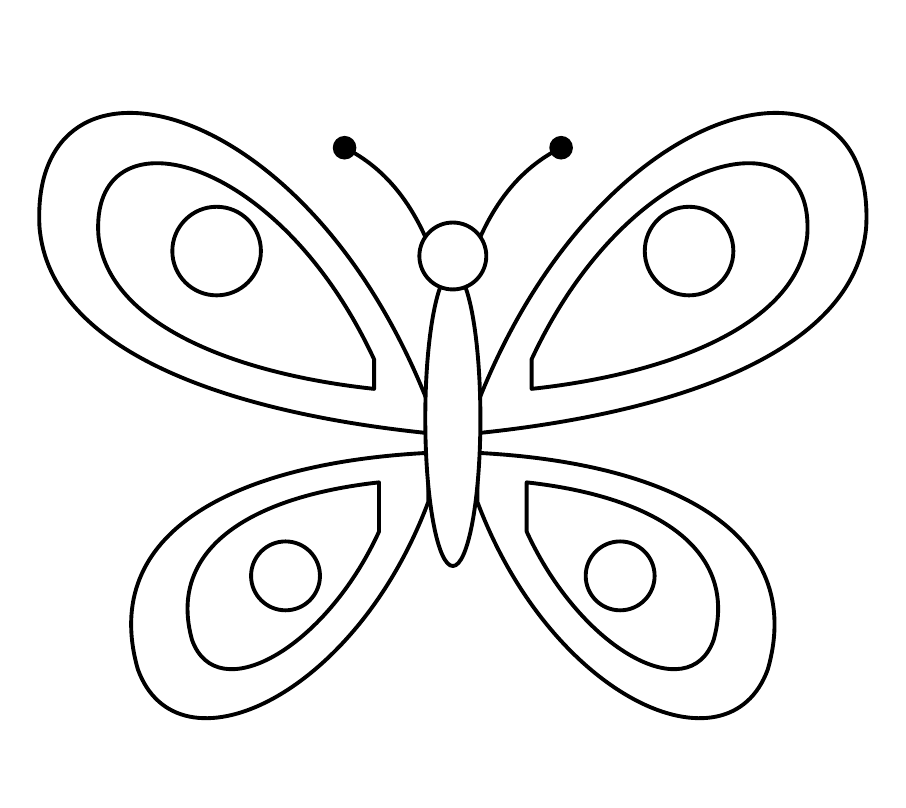
\begin{tikzpicture}[line width=1.4pt, line cap=round, line join=round, scale=1.25]
  \foreach \s in {1,-1} {
    \begin{scope}[xscale=\s]
      % el ala de arriba y su borde
      \filldraw[fill=white] (0.25,0.4) .. controls (1.5,3.6) and (4.3,4.2) .. (4.2,2.2)
        .. controls (4.1,0.9) and (2.2,0.3) .. (0.25,0.1) -- cycle;
      \draw (0.8,0.85) .. controls (1.8,3.0) and (3.7,3.4) .. (3.6,2.1)
        .. controls (3.5,1.2) and (2.2,0.7) .. (0.8,0.55) -- cycle;
      \filldraw[fill=white] (2.4,1.95) circle (0.45);
      % el ala de abajo y su borde
      \filldraw[fill=white] (0.25,-0.1) .. controls (2.2,-0.2) and (3.6,-0.9) .. (3.2,-2.3)
        .. controls (2.8,-3.4) and (1.0,-2.6) .. (0.25,-0.6) -- cycle;
      \draw (0.75,-0.4) .. controls (2.1,-0.55) and (2.9,-1.1) .. (2.65,-2.0)
        .. controls (2.4,-2.7) and (1.3,-2.1) .. (0.75,-0.9) -- cycle;
      \filldraw[fill=white] (1.7,-1.35) circle (0.35);
      % la antena
      \draw (0.08,1.5) .. controls (0.3,2.4) and (0.7,2.8) .. (1.1,3.0);
      \fill (1.1,3.0) circle (0.12);
    \end{scope}
  }
  % el cuerpo
  \filldraw[fill=white] (0,0.25) ellipse (0.28 and 1.5);
  \filldraw[fill=white] (0,1.9) circle (0.34);
\end{tikzpicture}
